


\begin{figure*} [t]
\center
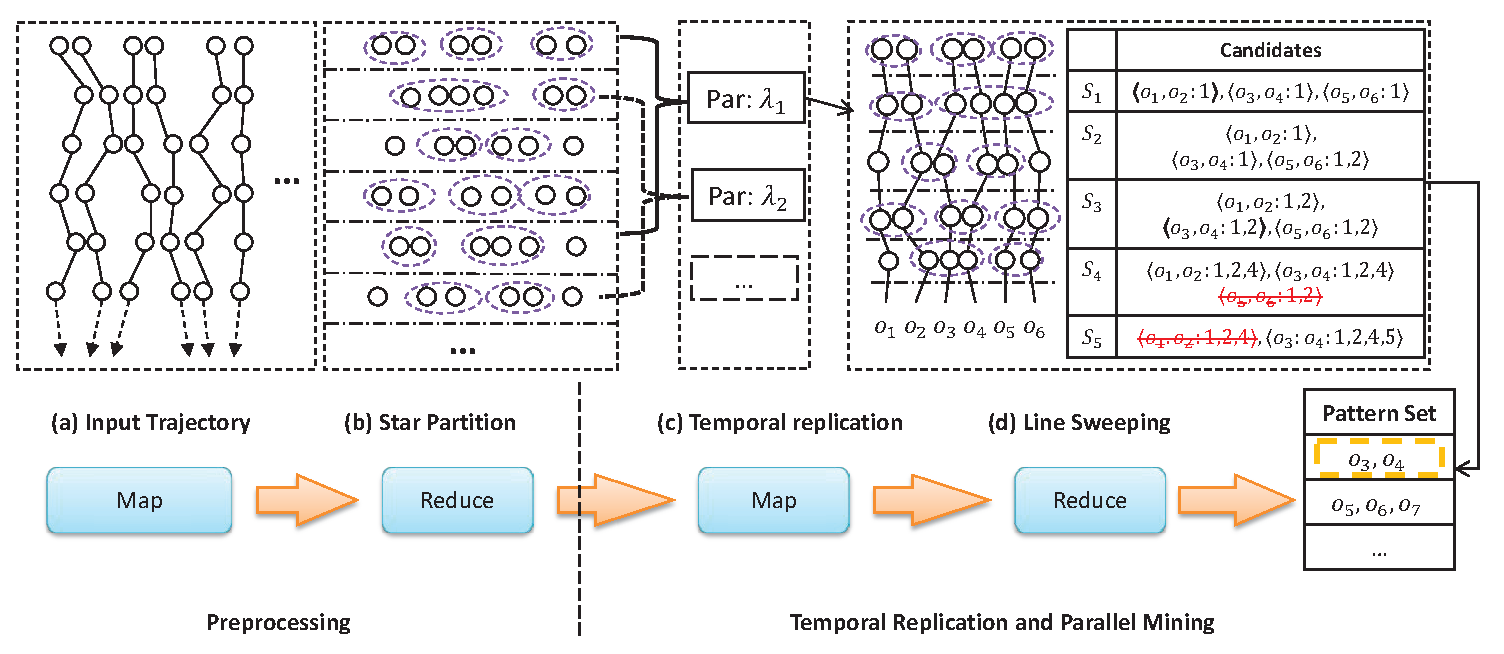
\includegraphics[width=\textwidth]{trm.eps}
\caption{Work flow of Temporal Replication and Mining. (a)(b) correspond to the first map-reduce cycle which clusters objects in each snapshot;  (c)(d) correspond to the second map-reduce cycle which uses temporal replication to mine GCMP in parallel.}
\label{fig:trm}
\end{figure*}

\section{Baseline: Temporal Replication and Parallel Mining}
\label{sec:trm}
In this section, we propose a baseline solution that resorts to MapReduce (MR) as a general, parallel and scalable paradigm for GCMP pattern mining. The framework, named \textit{temporal replication and parallel mining} (TRPM), is illustrated in   Figure~\ref{fig:trm}. There are two cycles of map-reduce jobs connected in a pipeline manner. The first cycle deals with spatial clustering in each snapshot, which can be seen as a preprocessing step for the subsequent pattern mining. In particular, the timestamp is treated as the key in the map phase and objects within the same snapshot are clustered (DBSCAN or disk-based clustering) in the reduce phase. Finally, the reducers output clusters of objects in each snapshot, represented by a list of $\langle t,S_t \rangle$ pairs, where $t$ is the timestamp and $S_t$ is a set of clustered objects at snapshot $t$. 

Our focus in this paper is the second map-reduce cycle of parallel mining, which essentially consists of two key questions to solve. The first is how to employ effective data partitioning such that the mining can be conducted independently; and the second is how to efficiently mine the valid patterns within each partition. 


It is obvious that we cannot simply split the trajectory database 
into disjoint partitions because a GCMP pattern requires $L$-consecutiveness 
and the corresponding segments may cross multiple partitions. 
Our strategy is to use data replication to enable parallel mining. 
Each snapshot will replicate its clusters to $\eta-1$ preceding snapshots.
In other words, the partition for the snapshot $S_t$ contains clusters 
in $S_t$, $S_{t+1}\ldots,S_{t+\eta-1}$. 
Determining a proper $\eta$ is critical in ensuring the
correctness and efficiency of TRPM. If $\eta$ is too small, 
certain cross-partition patterns may be missed. 
If $\eta$ is set too large, expensive network communication and 
CPU processing costs would be incurred in the map and reduce phases respectively. Our objective is to find an $\eta$ that is not large but can guarantee correctness.


In our implementation, we set $\eta = (\lceil \frac{K}{L} \rceil - 1)*(G-1)+K+L-1$. Intuitively, $K$ timestamps generates at most $\lceil \frac{K}{L} \rceil - 1$ gaps as the length of each $L$-consecutive segment is at least $L$. Since the gap size is at most $G-1$, $(\lceil \frac{K}{L} \rceil - 1)*(G-1)$ is the upper bound of timestamps allocated to gaps. The remaining part $K+L-1$ is used to capture the upper bound allocated for the $L$-consecutive segments. We formally prove that $\eta$ can guarantee correctness.


\eat{
Before moving on to find the value of $\eta$, 
we first use $\rho_{G,L,K}(T)$ to define the \emph{min-spanned valid subsequence} 
of a sequence $T$. In simple words, $\rho_{G,L,K}(T)$ is the 
subsequence of $T$ with the smallest range and is valid wrt. $K,L,G$. 
%Let $\eta_T$ denote
%the range of $\rho_{G,L,K}(T)$.
To guarantee that no valid patterns are missing, $\eta$ needs
to be greater than the range of $\rho_{G,L,K}(T)$ for any
valid sequence $T$. To see this, consider an arbitrary valid sequence $T$.
Since each partition contains $\eta$ snapshots,
if $\eta \geq \range(\rho_{G,L,K}(T))$ holds, $\rho_{G,L,K}(T)$ must be completely located in one partition. Therefore, the patterns associated with $T$ would not be missing.
Formally, $\eta$ can be computed as:
\begin{equation}
\eta = \max\{\range(\rho_{G,L,K}(T)) | T \text{ is valid wrt. } G,L,K\}
\end{equation}

Directly compute such $\eta$ is challenging. However,
we provide the following theorem which states a bounded estimation on $\eta$: 
}



\begin{theorem}
\label{THM:RP_ETA}
$\eta = (\lceil \frac{K}{L} \rceil - 1)*(G-1)+K+L-1$ guarantees that no valid pattern is missing.
\end{theorem}
\begin{proof}
Given a valid pattern $P$, consider its time sequence $T$. Since $T$ is valid wrt. $G,L,K$,
we can always find a minimum valid subsequence of $T$ denoted as $T'$.
We prove our theorem by showing that $\range(T') \leq \eta$.
Since $T'$ is valid, we may view $T'$ as interleaving 
segments and gaps. That is $T'$ can be written as $l_1,g_1,\ldots,l_{n-1},g_{n-1},l_n$ ($n \geq 1$),
where $l_i$ is a segment and $g_i$ is a gap. Then, $\range(T')$
is calculated as $\Sigma_{i=1}^{i=n}|l_i| + \Sigma_{i=1}^{i=n-1} |g_i|$. Since $T'$
is valid, then $\Sigma_{i=1}^{i=n}|l_i| \geq K$. As $T'$ is minimum, if we remove the 
last $l_n$, the resulting sequence should not be valid. Let $K' = \Sigma_{i=1}^{i=n-1}|l_i|$, which
is the size of the first $(n-1)$ segments of $T'$. Then, $K' \leq K-1$.
Note that every $|l_i| \geq L$, thus $n \leq \lceil \frac{K'}{L} \rceil \leq \lceil \frac{K}{L} \rceil $. By
using the fact that every $|g_i| \leq G-1$, we achieve $\Sigma_{i=1}^{i=n-1} |g_i| \leq (n-1)(G-1)
\leq (\lceil \frac{K}{L} \rceil -1)(G-1)$. Next, consider the difference between $K$ and $K'$. Let 
$\Delta = K- K'$. To ensure $T'$'s minimum validity, $l_n$ must equal to $\min(L, \Delta)$.
Then, $\Sigma_{i=1}^{i=n}|l_i| = K' + l_n = K - \Delta + \min(L, \Delta) \leq K - 1 + L$. The last
inequality dues to the fact that $\Delta \geq 1$.
Therefore, $\range(T') \leq \eta$. It follows that, for every valid pattern $P$, there must
exists a partition $\lambda$ with size $\eta$, such that $P$ is also valid in $\lambda$. This proves our theorem.
\end{proof}

Note that Theorem~\ref{THM:RP_ETA} does not state the optimal value of $\eta$
for a given $G,L,K$. However, for any $G,L,K$, $\eta$ does not differ from
the optimal value by at most $L-1$. To see this, for any $G,L,K$, we can
generate a sequence $T$ by repeating the following pattern, a $L$-segment followed by $G$-gap. 
The repetition stops when $|T|\geq K$. Apparently $T$ is valid wrt. $G,L,K$.
It is easy to see that $T$ is minimal valid subsequence of itself, then $\eta^*  \geq \range(T) \geq (\lceil \frac{K}{L}\rceil -1)(G-1) + K$.
Therefore $\eta-\eta^* \leq L-1$.


\eat{
In order to formally compute the minimum value of $\eta$,
we enforce the
following statement on $\eta$:
%I HAVE NO IDEA WHAT YOU ARE TALKING ABOUT STARTING FROM HERE!!!
 \emph{Let $T'$ be the \emph{shortest} 
valid subsequence (wrt. $K,L,G$) of a valid temporal sequence $T$. 
Then, $\eta$ needs to be the upper bound for all $T'$ among all valid temporal sequences to ensure the completeness.} 
Finding the \emph{minimum} $\eta$ is not
straightforward. We notice the minimum $\eta$ is related to the temporal
parameters $K,L,G$ by making the following observation on $G=1$:








\emph{
Let $T$ be an arbitrary valid temporal sequence. Since $G$ equals to 1,
$T$ can be represented as $T=(t_1, t_2,...,t_m)$, where
$t_i +1 = t_{i+1}$ and $m \geq K$. Let $T' = (t_1,...,t_k)$, $T'$ is the shortest
valid temporal sequence of $T$. Note that $T'$ is fully contained
in the partition $\lambda_{t_1} = \{S_{t_1},...,S_{t_k}\}$, therefore it can be
mined in $\lambda_{t_1}$. 
Since $T$ is an arbitrary valid temporal sequence, the minimum $\eta$ is thus $K$.
}

Inspired by the observation, we generalize the relationship between
the minimum $\eta$ and temporal parameters using the following theorem:

\begin{theorem}
\label{THM:RP_ETA}
The minimum $\eta$ to ensure the completeness of the temporal replication is:
\[
   \eta = 
\begin{cases}
    (\lceil \frac{K}{L} \rceil -1)*(G-1)+2K -2, & \text{if } G \geq 2\\
    K,              & \text{if } G = 1
\end{cases}
\]
, where $K,L,G$ are the temporal parameters.
\end{theorem}

\begin{proof}
When $G = 1$, we have demonstrated $\eta=K$
in the above observation. When $G \geq 2$, we compute $\eta$ as follows:
any $T'$ can be viewed as $n$ consecutive segments with sizes $l_1,..,l_n$
and $n-1$ gaps with sizes $g_1,...,g_{n-1}$.
Since $\eta$ is the upper bond among all $T'$s, $\eta$ can be formulated 
as follows:
\begin{equation}
\eta = \max_{n,l_i,g_i} \{ \Sigma_{i=1}^{i=n} l_i + \Sigma_{i=1}^{i=n-1} g_i \}
\end{equation}
With the following constraints: (1)$\forall l_i, L \leq l_i \leq K-1$; (2)
$\forall g_i, 1 \leq g_i \leq G-1 $; (3) $\Sigma_{i=1}^{i=n} l_i \geq K$ and
(4) $\Sigma_{i=1}^{i=n-1}l_i  \leq K-1$. Constraints (1)(2)(3) due to the 
validity of $T'$ and $G\geq 2$ (4) is because $|T'|$ is minimum.
Based on (1)(3)(4), we can derive (5):  $n \in [1, \lceil \frac{K}{L} \rceil]$.
Constraints (1)-(5) form a convex polygon and $\eta$ is monotone
increasing wrt. $n, l_i, g_i$, therefore, the maximum value of $\eta$ is taken at the upper boundaries
where $g_i = G-1$, 
$\Sigma_{i=1}^{i=n-1}l_i = K-1$, $l_i = K-1$
and $n = \lceil \frac{K}{L} \rceil$. This leads to  $\eta = (\lceil \frac{K}{L} \rceil -1)*(G-1)+2K -2$.
\end{proof}
}

Based on the above theorem, during TRPM, every consecutive $\eta$ snapshots
form a partition. In other words, each snapshot $S_t$ corresponds to a partition $\lambda_t=\{S_t,...,S_{t+\eta-1}\}$. 
Our next task is to design an efficient pattern mining strategy within each partition. 
Since we have a partition $\lambda_t$ for every snapshot $S_t$,
we only need to report the patterns that appears in $S_t$ for $\lambda_t$. This would largely
reduce the overlapping computation between different partitions. To facilitate the goal,
%
%Since we have a partition $\lambda_t$ for every snapshot $S_t$, in the reduce phase, we only need to mine the patterns whose object set is in $S_t$ for partition $\lambda_t$.
%
%
we propose a \emph{line-sweep} algorithm. In brief, we treat clusters in $S_t$ as initial candidate patterns.
Then, we grow a candidate by intersecting it with clusters from next snapshots. When every snapshot is examined,
we output all valid candidate patterns.

The detail of \emph{line-sweep} is presented in Algorithm~\ref{algo:line-sweep}. We keep a candidate set $\mathbf{C}$ (Line~\ref{code:ls-can-set}) during the sweeping. In the beginning, 
all clusters in $S_t$ with sizes greater than $M$ form the initial candidates (Lines~\ref{code:ls-init-start}-\ref{code:ls-init-end}). Our algorithm then sequentially sweeps each snapshots (Lines~\ref{code:ls-sweep-starts}-\ref{code:ls-sweep-ends}).
During sweeping snapshot $S_j$, candidates in $\mathbf{C}$ join with clusters in $S_j$ to form new candidates (Lines~\ref{code:ls-join-start}-\ref{code:ls-join-ends}). 
%The join of candidate $c$ and cluster $s$ creates a
%new candidate $c'$ (Line~\ref{code:ls-join}).  
After sweeping the entire partition, valid candidates in $\mathbf{C}$
are reported (Line~\ref{code:ls-valid-check}). 
It is notable that $\mathbf{C}$ continuously grows as we sweeping, thus we use three pruning rules to reduce the size 
of $\mathbf{C}$. First, when sweeping snapshot $S_j$, new candidates with objects set less than $M$ are pruned (Line~\ref{code:ls-m-prun}). Second, after joined with all clusters in $S_j$, 
candidates in $\mathbf{C}$ with max time sequences no greater than $j-G$ are pruned (Lines~\ref{code:ls-g-prune-starts}-\ref{code:ls-g-prune-ends}). Third, candidates in $\mathbf{C}$ with the size of first segment less than $L$
are pruned (Lines~\ref{code:ls-l-prune-starts}-\ref{code:ls-l-prune-ends}). With the three pruning rules, the size
of $\mathbf{C}$ could be largely reduced.

%After join, there are two prunings. First, 
%all new candidates with objects set less than $M$ are pruned (Line~\ref{code:ls-m-prun}). Second,
%existing candidates with max time sequences no greater 
%than $j-G$ are pruned (Line~\ref{code:ls-m-prun}). 
% 
%
%During the sweeping, candidates in $\mathbf{C}$ join with $S_j$.
%
% Initially, all the clusters 
%
%During scanning, a set of pattern candidates is maintained.
%When all snapshots are scanned, the remaining candidates are the true patterns.
%The detail of LSM is presented in Algorithm~\ref{algo:line-sweep}.
%A candidate set $C$ is maintained throughout the algorithm(line~\ref{code:ls-can-set}). $C$
%is initialized by inserting clusters at $S_t$ (lines~\ref{code:ls-init-start}-\ref{code:ls-init-end}).
%During scanning snapshot $S_j$, candidates in $C$ are joined with clusters at $S_j$. In
%the join, a candidate grows its temporal sequence while potentially reduces its object set. After the join,
%false patterns are deleted (line~\ref{code:ls-remove}). 
%Note that the size of $C$ is always decreasing, therefore the complexity of LSM $\lambda_t$ is $O(\eta|S_t||\overline{S}|)$,where $|\overline{S}|$ is the average snapshot size in $\lambda_t$.
\begin{algorithm}[t]
\caption{Line Sweep Mining}
\label{algo:line-sweep}
\begin{algorithmic}[1]
\Require $\lambda_t = \{S_t, ..., S_{t+\eta-1}\}$
\State{$\mathbf{C} \gets \{\}$} \Comment{Candidate set} \label{code:ls-can-set}
\For{$s \in S_t$} 
\label{code:ls-init-start}
\State $\mathbf{C}$.add($\langle s, t \rangle $), if $|s| \geq M$
\EndFor
\label{code:ls-init-end}
\ForAll{$S_j \in \{S_{t+1},\ldots,S_{t+\eta-1}\}$} \label{code:ls-sweep-starts}
	\State $\mathbf{N} \gets \{\}$
	\ForAll {$(c,s) \in \mathbf{C} \times S_j$} \label{code:ls-join-start}
		\State {$c' \gets \langle c.O \cap s.O, c.T \cup \{j\} \rangle$} \label{code:ls-join}
		\If {$c'.T$ is valid} 
			\State output $c'$
		\Else
			\State $\mathbf{N}.\mathtt{add}(c')$, if  $|c'.O| \geq M$ \label{code:ls-m-prun}	
		\EndIf
	\EndFor \label{code:ls-join-ends}
	\ForAll {$c \in \mathbf{C}$}
		\If{$j-\max(c.T)\geq G$}\label{code:ls-g-prune-starts}
			\State $\mathbf{C}.\mathtt{remove}(c)$ 
			\State output $c$, if $c$ is a valid pattern
		\EndIf  \label{code:ls-g-prune-ends}
		\If{$c$'s first segment is less than $L$}\label{code:ls-l-prune-starts}
			\State $\mathbf{C}.\mathtt{remove}(c)$ 
		\EndIf\label{code:ls-l-prune-ends}
	\EndFor
	\State $\mathbf{C}.\mathtt{addAll}(\mathbf{N})$
\EndFor\label{code:ls-sweep-ends}
\State output valid patterns in  $\mathbf{C}$  \label{code:ls-valid-check}
\end{algorithmic}
\end{algorithm}
The complete picture of temporal replication and parallel mining is summarized in Algorithm~\ref{algo:trm_overview}. We illustrate the workflow of TRPM method using Figure~\ref{fig:trm} (c)(d) with pattern
parameters $M=2, K=3, L = 2, G=2$. By Theorem~\ref{THM:RP_ETA}, $\eta$ is calculated
as $(\lceil \frac{K}{L} \rceil-1) *(G-1)+2K - 2 = 5$. Therefore, 
in Figure~\ref{fig:trm} (c), every $5$ consecutive snapshots are combined 
into a partition in the map phase. In Figure~\ref{fig:trm} (d), a line sweep
method is illustrated for partition $\lambda_1$. Let $C_i$ be the candidate set
during sweeping snapshot $S_i$.
Initially, $C_1$ contains patterns whose object set is in snapshot $S_1$.
As line sweeps, the patterns in $C_i$ grows. At snapshot $S_4$, the candidate
$\{o_5,o_6\}$ is removed. This is because the gap between its latest timestamp (i.e., $2$)
and the next scanning timestamp (i.e., $5$) is $3$, which violates the $G$ constraint.
Next, at snapshot $S_5$, the candidate $\{o_1,o_2\}$ is removed. This is
because its local consecutive timestamps $\{4\}$ has only size $1$,
which violates the $L$ constraint.
Finally, $\{o_3,o_4\}$ is the qualified pattern and is outputted. Note that the minimum $\eta$
under this setting is $5$. If $\eta$ is chosen as $4$, the pattern $\{o_3,o_4\}$ would be excluded. 

\begin{algorithm}[h]
\caption{Temporal Replication and Parallel Mining}
\label{algo:trm_overview}
\begin{algorithmic}[1]
\Require list of $\langle t, S_t \rangle$ pairs
\State $\eta \gets (\lceil \frac{K}{L} \rceil -1)*(G-1)+K+L-1$
\State {---Map Phase---}
\label{code:trm-map-start}
\ForAll{$\langle t, S_t \rangle$}
	\ForAll{$i \in 1...{\eta-1}$}
		\State emit a $\langle \max(t-i,0), S_t \rangle$ pair
	\EndFor  
\EndFor
\label{code:trm-map-end}
\State {---Partition and Shuffle Phase---}
\label{code:trm-par-start}
\ForAll{$\langle t, S \rangle$ pair} 
\State group-by $t$, emit a $\langle t, \lambda_t\rangle$
\State where $\lambda_t = \{S_t, S_{t+1}, .. S_{t+\eta-1}\} $
\EndFor
\label{code:trm-par-end}
\State {---Reduce Phase---}
\label{code:trm-red-start}
\ForAll{$\langle t,\lambda_t \rangle$}
\State lineSweepMining($\lambda_t$)
\label{code:trm-red-end}
\EndFor
\end{algorithmic}
\end{algorithm}

